\section{Sistemi di transizione etichettati - (LTS)}
La verifica dei sistemi si serve di stumenti automatici. Quindi, viene naturale farsi la seguente domanda:

\begin{center}
\emph{come possiamo descrivere un sistema software?}
\end{center}

Ovviamente non possiamo utilizzare il linguaggio naturale, poichè esso è un linguaggio ambiguo. Abbiamo bisogno di un linguaggio formale che ci permetta di descrivere un sistema software senza ambiguità e che abbia una semantica ben definita. In altre parole abbiamo bisogno di un \emph{modello} del sistema. Per venire incontro a queste necessità sono stati ideati i sistemi di transizione etichettati, in inglese \emph{Label Transition System - (LTS)}. Gli LTS sono una generalizzazione degli \emph{automi a stati finiti - (FSM)} \cite{NoteProf}, infatti un LTS a differenza di un FSM ha le seguenti proprietà:

\begin{itemize}
 \item il numero degli stati di un LTS non è necessariamente finito;
 \item l'insieme delle transizioni di un LTS non è necessariamente finito.
\end{itemize}

\subsection{Definizione formale}
Un \emph{sistema di transizione etichettato} $TS$ è una sestupla 

\begin{equation}
TS\ =\ \langle\ S,\ Act,\ \rightarrow,\ I,\ AP,\ L\ \rangle
\end{equation}

\noindent dove:

\begin{itemize}
 \item $S\ $ è l'\emph{insieme degli stati} del sistema
 
 \item $Act\ $ è l'insieme finito dei simboli che rappresentano le \emph{azioni}. Le azioni possono essere di due tipi: \emph{interne} o \emph{esterne};
 
 \item $\rightarrow\ \subseteq S \times Act \times S\ $ è una relazione ternaria detta \emph{relazione di transizione} ed è un sottoinsieme del prodotto cartesiano $S \times Act \times S$.
 
 \textbf{Esempio:} $(p, \lambda, q) \in \rightarrow \ $ si può scrivere come $p\ \xrightarrow{\lambda}\ q$ e significa che il processo $p$ esegue l'azione $\lambda$ e si comporta come il processo $q$;
 
 \item $I\ \subseteq S $ è l'\emph{insieme degli stati iniziali};
 
 \item $AP\ $ è l'\emph{insieme delle proprietà atomiche}. Una proprietà è un predicato $P$ che associa ad ogni elemento $x$ o insieme $X$ un valore di verità;
 
 \item $L\ $ è la \emph{funzione di labeling} o sistema di etichettatura. È definita come
 \begin{equation}
  L:\ S \rightarrow 2^{AP}
 \end{equation}
 Il dominio della funzione $L$ è l'insieme degli stati del sistema $S$. Il codominio è l'insieme delle parti delle proprietà atomiche $AP$. Si ricorda che l'insieme delle parti o insieme potenza di un insieme $A$ è l'insieme
 \begin{equation}
  2^A=\ \{ X\ |\ X \subseteq A \}
 \end{equation}
 ovvero l'insieme di tutti i sottoinsiemi di $A$.
 Per ogni stato $s \in S$, l'insieme $L(s)$ è l'insieme di tutte le proposizione atimiche valide in $s$.
 
\end{itemize}

\subsubsection*{Esempio}

In figura \ref{fig:esempio-LTS} è mostrato il sistema di transizione $TS\ = \langle\ S,\ Act,\ \rightarrow , I, \dots \rangle$ di una macchina del caffè. Abbiamo che:

\begin{itemize}
 \item l'insieme degli stati del sistema:  S = \{ Ready,\ Select,\ Coffee,\ Tea \};
 \item l'insieme delle azioni:  Act = \{ Insert\_coin,\ Select\_coffee,\ Select\_tea,\ Supply\_coffee,\ Supply\_tea \};
 \item la relazione di transizione:
 
$ \rightarrow\ $= \{(Ready, Insert\_coin, Select),\ (Select, Select\_coffee, Coffee),\ (Select, Select\_tea, Tea),
 \  (Tea, Supply\_tea, Ready),\ (Coffee, Supply\_coffee, Ready)\}

\item l'insieme degli stati iniziali: I = \{ Ready \}
\end{itemize}


\begin{figure}[ht]

\begin{center}

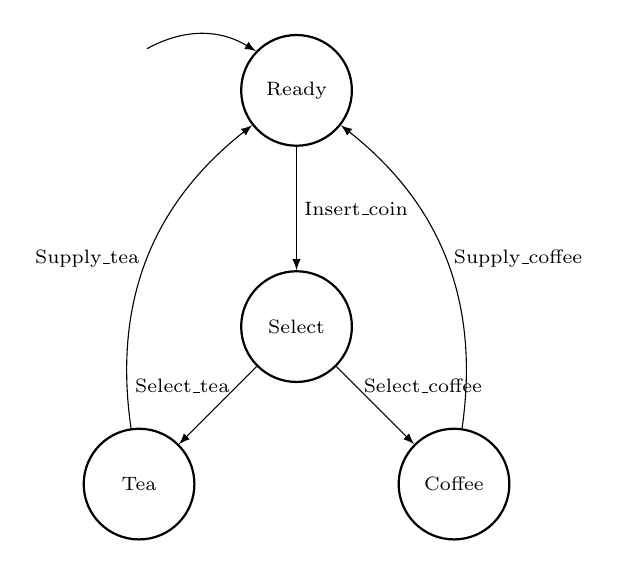
\begin{tikzpicture}

  \tikzstyle{node}=[shape=circle,inner sep=3pt, minimum size=40pt ,draw,thick]

  \tikzstyle{mpr}=[shape=circle,inner sep=1.5pt,draw,thick, fill=black]

  \tikzstyle{source}=[shape=rectangle,draw,dashed]

  \tikzstyle{lineDecorate}=[near start, -latex,draw]

  \tikzstyle{lineDecorateSource}=[-latex,draw,dashed, arrows=<->]

%[lineDecorate/.style={-,thick}, nodeDecorate/.style={shape=circle,inner sep=1.5pt,draw,thick}]

\scriptsize

%% nodes or vertices

\node (S) at (-2,5.5) {};

\node (A)[node] at (0,5) {Ready};

\node (B)[node] at (0,2) {Select};

\node (C)[node] at (-2,0) {Tea};

\node (D)[node] at (2,0) {Coffee};





%% edges or lines anchor=east

\path[->]

	(C) edge[lineDecorate, bend left] node[anchor=east, midway] {Supply\_tea} (A)

	(D) edge[lineDecorate, bend right] node[anchor=west, midway] {Supply\_coffee} (A)


;
%lineDecorateSource tratteggiata

\path[->]
	(S) edge[lineDecorate, bend left] node[anchor=west] {} (A)
	
	
	(A) edge[lineDecorate] node[anchor=west, midway] {Insert\_coin} (B)

	(B) edge[lineDecorate] node[anchor=west] {Select\_coffee} (D)

	(B) edge[lineDecorate] node[anchor=east] {Select\_tea} (C)

;
\end{tikzpicture}

\caption{Esempio di uno schema LTS per l'automa di una macchina del caffè.}

\label{fig:esempio-LTS}

\end{center}

\end{figure}




\subsection{Cammino o computazione}
In un LTS un \emph{cammino} ( o \emph{computazione}) $\pi$ è una sequenza finita (o infinita) della forma:

 \begin{equation}
  s_0 \lambda_0 s_1 \lambda_1 s_2 \lambda_2 \dots \dots \lambda_{n-1} s_n 
 \end{equation}
 
 \noindent dove $ \forall\ i,\ \exists\ s_i\ \xrightarrow{ \lambda_i }\ s_{i+1} \in\ \rightarrow\ $.
 
 Equivalentemente un cammino può essere scritto nelle seguenti forme:
 
 \begin{equation}
  (\ s_0,\ \lambda_0,\ s_1\ ), (\ s_1,\ \lambda_1,\ s_2\ ),\ \dots \dots, (\ s_{n-1},\ \lambda_{n-1},\ s_n\ )
 \end{equation}
 oppure
 \begin{equation}
  s_0\ \xrightarrow{ \lambda_0 }\ s_{1}\ \xrightarrow{ \lambda_1 }\ s_{2}\ \dots \dots \xrightarrow{ \lambda_{n-1} }\ s_{n}
 \end{equation}
 
\noindent Il cammino nullo è la sequenza vuota.
 \\
 
 Una cammino si dice \emph{iniziale} se $s_0\ \in I$.  
 Una cammino si dice \emph{massimale} se $s_n$ è uno stato terminale, oppure se è un cammino infinito.
 
 Uno stato $s\ \in\ S$ è \emph{raggiungibile} in un $TS\ =\ \langle\ S,\ Act,\ \rightarrow,\ I,\ AP,\ L\ \rangle$ se esiste un cammino finito ed iniziale tale che
 
  \begin{equation}
  s_0\ \xrightarrow{ \lambda_0 }\ s_{1}\ \xrightarrow{ \lambda_1 }\ s_{2}\ \dots \dots \xrightarrow{ \lambda_{n-1} }\ s_{n}\ =\ s
 \end{equation}
 
 Adesso consideriamo $TS\ = \langle\ S,\ Act,\ \rightarrow, \dots \rangle$. Indicheremo con:
 
 \begin{itemize}
  \item $\ Post( s, \lambda )\ = \{\ s' \in S\ |\ s\ \xrightarrow{ \lambda }\ s'\ \}\ $ ovvero l'insieme di tutti gli stati $s' \in S$ raggiungibili dallo stato $s \in S$ facendo un'azione $\lambda\ \in\ Act$;
  
  \item $\ Post(s) = \bigcup_{\lambda\ \in\ Act}^{} Post( s, \lambda )\ $ l'insieme di tutti gli stati raggiungibili dallo stato $s \in S,\ \forall \lambda \in Act$;
  
  \item $\ Preset( s, \lambda )\ = \{\ s' \in S\ |\ s'\ \xrightarrow{ \lambda }\ s\ \}\ $ l'insieme di tutti gli stati che attraverso un'azione $\lambda\ \in\ Act$ vanno nello stato $s \in S$;
  
  \item $\ Preset( s )\ = \bigcup_{\lambda\ \in\ Act}^{} Preset( s, \lambda )\ $ l'insieme di tutti gli stati che evolvono nello stato $s \in S,\ \forall \lambda \in Act$.
 \end{itemize}
 
\textbf{Stallo}

Un sistema si dice che è in \emph{stallo} (o in deadlock) quando non può eseguire nessuna azione e lo stato in cui si trova non è uno stato terminale.
\\
 
\textbf{Osservazioni:} un sistema è in stallo se $\ Post(s) = \emptyset $. Inoltre, se $s \in S$ è uno stato terminale, allora $\ Post(s) = \emptyset $.
\\

\clearpage

\subsection{Determinismo e non determinismo}
Un sistema si dice \emph{non deterministico} se può comportarsi in due o più modi differenti con lo stesso input. In formule:

\begin{equation}
 \exists \, (s, \lambda)\ :\ \rvert Post( s, \lambda ) \rvert > 1
\end{equation}

Un sistema si dice \emph{deterministico} se per ogni stato del sistema, esiste una e una sola azione tale che è possibile determinare in modo univoco lo stato successivo. In formule:

\begin{equation}
 \forall s \in S,\ \exists! \, \lambda \in Act\ :\ \rvert Post( s, \lambda ) \rvert = 1
\end{equation}

Si possono avere due tipi di determinismo:

\begin{itemize}
 \item Action Determinism
 \item AP-Determinism
\end{itemize}

Un sistema è \emph{action deterministic} (deterministico rispetto alle azioni) allora
\begin{equation}
|I| \leq 1,\ \forall s \in S,\ \forall \lambda \in Act\ \Leftrightarrow\ \rvert Post( s, \lambda ) \rvert \leq 1
\end{equation}
ovvero, l'insieme degli stati iniziali deve avere cardinalità al più uno e per ogni coppia stato-azione, l'insieme degli stati successivi deve avere cardinalità al più uno.

Un sistema è \emph{AP-deterministic} (deterministico rispetto alle proprietà atomiche) allora
\begin{equation}
 |I| \leq 1,\ \forall s \in S,\ \forall \lambda \in Act\ \Leftrightarrow\ \rvert Post(s) \cap \{ s' \in S\ |\ L(s') = A \} \rvert \leq 1
\end{equation}
ovvero, l'insieme di tutti gli stati successivi allo stato $s$ intersecato con l'insieme degli stati che soddisfano la proprietà atomica $A$ ha cardinalità al più $1$.



 


 
